\begin{figure}[btp]
\small
    \centering
        \begin{tabular}{|l|l|l|l|}
        \hline
        \multicolumn{2}{|l|}{\multirow{2}{*}{D-Sub Connector}} & \multicolumn{2}{c|}{Goal}                                 \\ \cline{3-4} 
        \multicolumn{2}{|l|}{}                     & \multicolumn{1}{c|}{Perfect} & \multicolumn{1}{c|}{Noisy} \\ \hline \hline
        \multirow{3}{*}{Pure RL} & Dense & 16\% & 0\% \\ 
         & Images, SAC & 0\% & 0\% \\
          & Images, TD3 & 12\% & 12\% \\ \hline
        \multirow{1}{*}{RL + LfD} & Images & 52\% & 52\% \\  \hline
        \multirow{3}{*}{Residual RL} & Dense & \textbf{100\%} & 60\% \\ 
         & Images, SAC & \textbf{100\%} & \textbf{64\%} \\
          & Images, TD3 & 52\% &  52\% \\ \hline
        \multirow{1}{*}{Human} & P-Controller & \textbf{100\%} & 44\% \\   \hline
        \end{tabular}
        \hfill
        %\hspace{0.5cm}
        \begin{tabular}{|l|l|l|l|}
        \hline
        \multicolumn{2}{|l|}{\multirow{2}{*}{Model-E Connector}} & \multicolumn{2}{c|}{Goal}                                 \\ \cline{3-4} 
        \multicolumn{2}{|l|}{}                     & \multicolumn{1}{c|}{Perfect} & \multicolumn{1}{c|}{Noisy} \\ \hline \hline
        \multirow{3}{*}{Pure RL} & Dense & 0\% & 0\% \\ 
         & Images, SAC & 0\% & 0\% \\ 
         & Images, TD3 & 0\% & 0\% \\ \hline
        \multirow{1}{*}{RL + LfD} & Images & 20\% & 20\% \\  \hline
        \multirow{3}{*}{Residual RL} & Dense & \textbf{100\%} & \textbf{76\%} \\ 
         & Images, SAC &\textbf{100\%} & \textbf{76\%} \\ 
           & Images, TD3 & 0\% & 0\% \\ \hline
        \multirow{1}{*}{Human} & P-Controller & 52\% & 24\% \\   \hline
        \end{tabular}
        % \vspace{10pt}
    \caption{We report average success out of 25 policy executions after training is finished for each method. For noisy goals, noise is added in form of $\pm 1\,\mathrm{mm}$ perturbations of the goal location. Residual RL, particularly with SAC, tends to be the best performing method across all three connectors. For the \text{Model-E}~connector, only residual RL solves the task in the given amount of training time.}
    \label{fig:tables}
    % \vspace{-0.5cm}
\end{figure}

\section{Results}\label{sec:results}

We analyze the performance of policies learned with residual RL, as well as other methods, based on their ability to achieve the task goal, as well as the distance of the final object location to the goal pose over the course of training. To study the robustness of the learned policies, we also evaluate them in conditions where the goal connector position is perturbed, in order to understand the tolerance of RL policies to imprecise object placement.

\subsection{Vision-based Learning}
The results of the vision-based experiment are shown in Fig.~\ref{vision_based_distance_all}.
Our experiments show that a successful and consistent vision-based insertion policy can be learned from relatively few samples using residual RL. 

\begin{wrapfigure}{r}{0.5\linewidth}
    % \begin{figure}[t]
    \label{tab:goal_pertubation_USB}
    \renewcommand{\arraystretch}{1.0}
    \begin{center}
    \small
    \begin{tabular}{|l|l|l|l|}
    \hline
    
    \multicolumn{2}{|l|}{\multirow{2}{*}{USB Connector}} & \multicolumn{2}{c|}{Goal}                                 \\ \cline{3-4} 
    \multicolumn{2}{|l|}{}                     & \multicolumn{1}{c|}{Perfect} & \multicolumn{1}{c|}{Noisy} \\ \hline \hline
    
    \multirow{5}{*}{Pure RL}   
     & Dense & 28\% & 20\% \\ 
     & Sparse, \;SAC & 16\% & 8\% \\ 
     & Sparse, \;TD3 & 44\% & 28\% \\ 
      & Images, SAC & 36\% & 32\% \\ 
       & Images, TD3 & 28\% & 28\% \\ \hline
    \multirow{2}{*}{RL + LfD} & Sparse &\textbf{100\%} & 32\% \\ 
     & Images & 88\% & 60\% \\ \hline
    \multirow{5}{*}{Residual RL} & Dense &\textbf{100\%} & \textbf{84\%} \\ 
     & Sparse,\: SAC & 88\% &  \textbf{84\%}\\ 
     & Sparse,\: TD3 &\textbf{100\%} & 36\% \\
     & Images, SAC & \textbf{100\%} & 80\% \\
      & Images, TD3 &  0\%& 0\%\\
      \hline
    \multirow{1}{*}{Human} & P-Controller & \textbf{100\%} & 60\% \\   \hline
    \end{tabular}
    \end{center}
    \vspace{5pt}
    \caption{Average success rate on the USB insertion task. Residual RL and RL + LfD solve the task consistently. Moreover, residual RL stays robust under $\pm1$\text{mm} noise. }
    \label{fig:TableUSB}
    % \end{figure}
    % \vspace{-0.7cm}
\end{wrapfigure}

This result suggests that goal-specification through images is a practical way to solve these types of industrial tasks. Although image-based rewards are often very sparse and hard to learn from, in this case the distance between images corresponds to a relatively dense reward signal which is sufficient to distinguish the different stages of the insertion process.

Interestingly, during training with standard RL, the policy would sometimes learn to ``hack'' the reward signal by moving down in the image in front of or behind the socket. In contrast, the stabilizing human-engineered controller in residual RL provides sufficient horizontal control to prevent this. The initial controller also scaffolds the learning process, by providing a very strong initialization that requires the reinforcement learning algorithm to only learn the final phase of the insertion. This produces substantially better performance in conjunction with vision-based rewards.

\begin{wrapfigure}{r}{0.5\linewidth}
% \begin{figure}[tbp]
    \centering
        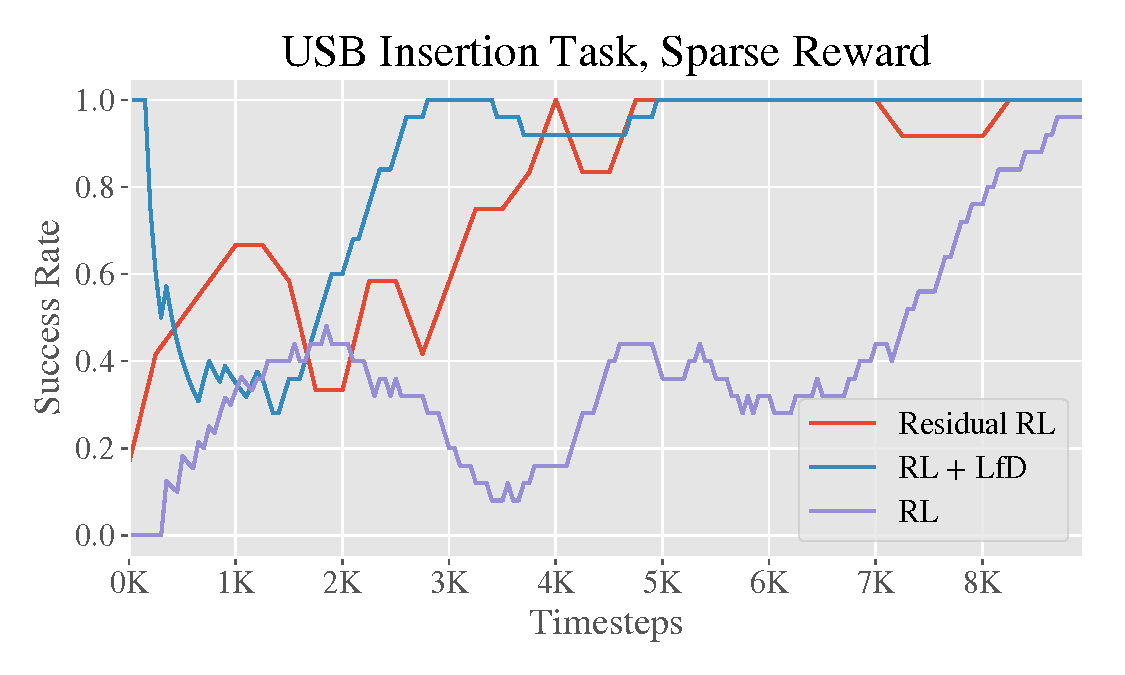
\includegraphics[width=0.99\linewidth]{insertion/newfigs/Sparse_success_all.pdf}
    \caption{Learning curves for solving the USB insertion task with a sparse reward. Final distance to goal is shown; lower is better. Residual RL and RL with learning from demonstrations both solve the task relatively quickly, while RL alone takes about twice as long to solve the task at the same performance. }
    \label{fig:SparseRewardsAll}
    \vspace{-1.0cm}
% \end{figure}
\end{wrapfigure}

\subsection{Learning From Sparse Rewards}

In this experiment, we compare these methods on the USB insertion task with sparse rewards. The results are reported in Fig.~\ref{fig:SparseRewardsAll}. All methods are able to achieve very high success rates in the sparse setting. 
This result shows that we can learn precise industrial insertion tasks in sparse-reward settings, which can often be obtained much more easily than a dense, shaped reward. 
In fact, prior work has found that the final policy for sparse rewards can outperform the final policy for dense rewards as it does not suffer from a misspecified objective \cite{andrychowicz2017her}.

\subsection{Perfect State Information}
The results of the experiment with perfect state information and dense rewards is shown in Fig.~\ref{fig:state_based_distance_all}. In this case, residual RL still outperforms standard RL, though the better-shaped reward enables standard RL to make more initial progress than with the other reward signals.
However, the hand-designed shaped reward function makes it harder for the policy to actually perform the full insertion, potentially because the more complex reward landscape provides other competing goals to the policy. The final performance with sparse rewards on the USB insertion task is substantially better.


\begin{figure}[tbp]
    \centering
    \resizebox{1.02\linewidth}{!}{
    \begin{subfigure}[b]{0.32\linewidth}
        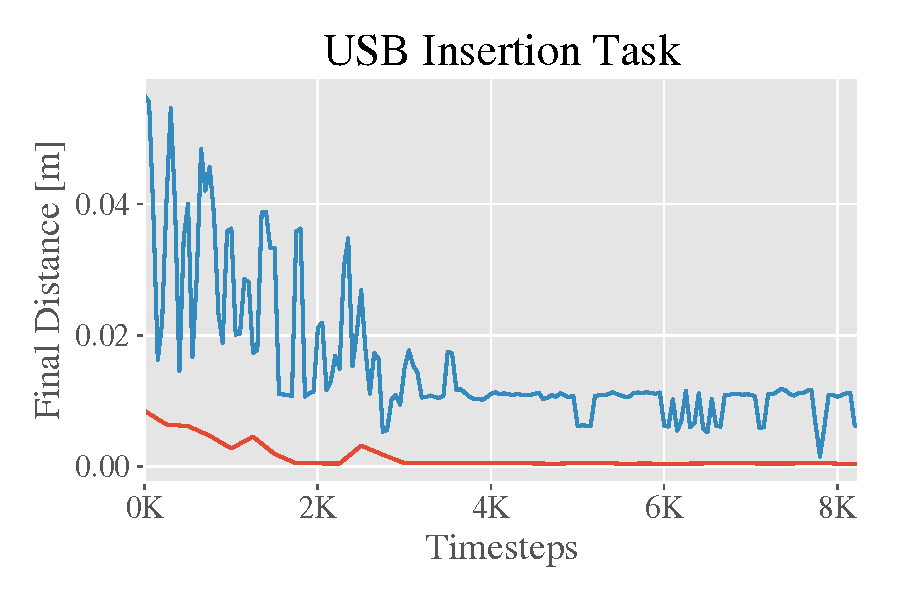
\includegraphics[width=0.99\linewidth]{insertion/newfigs/USB_state_distance.pdf}
    \end{subfigure}
    \begin{subfigure}[b]{0.32\linewidth}
        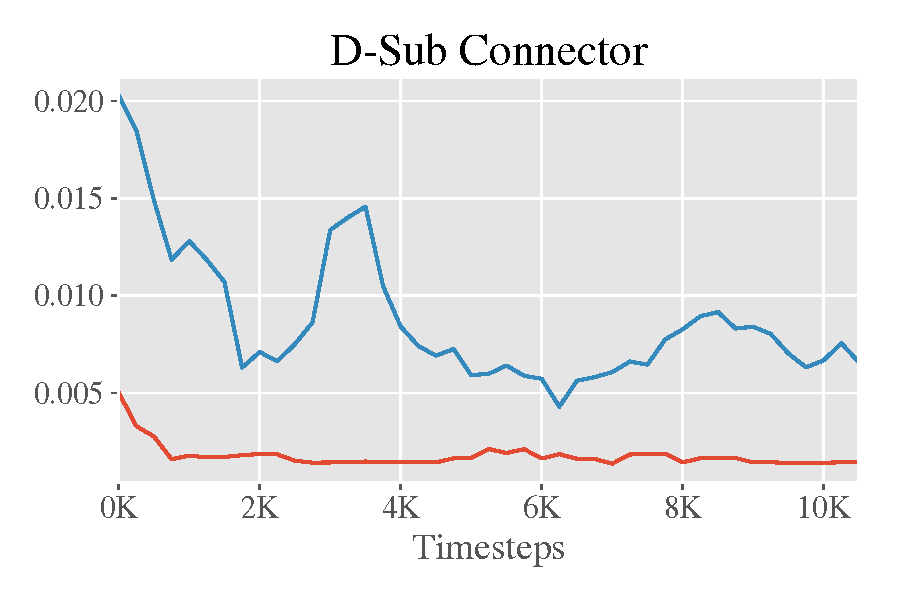
\includegraphics[width=0.99\linewidth]{insertion/newfigs/DSUB_states_distance.pdf}
    \end{subfigure}
    \begin{subfigure}[b]{0.32\linewidth}
        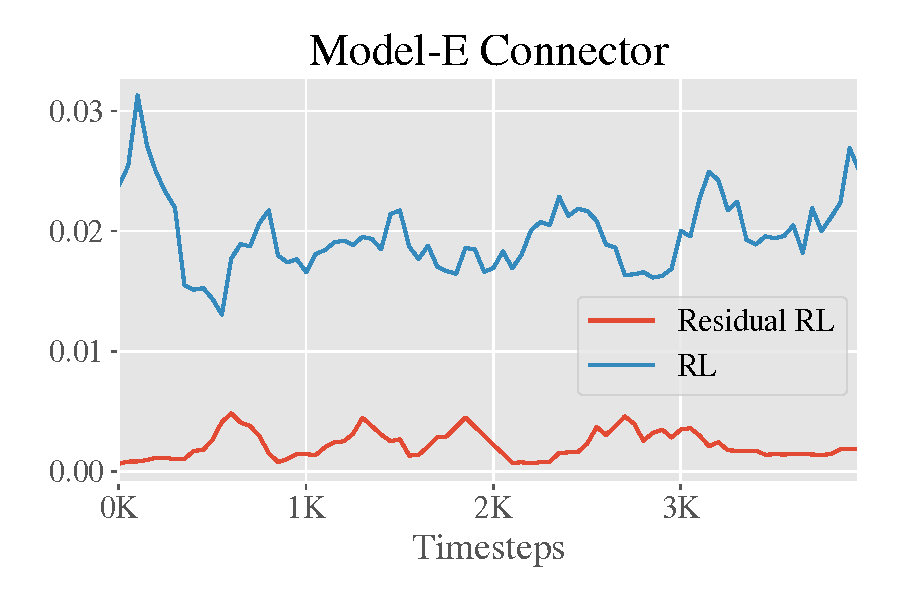
\includegraphics[width=0.99\linewidth]{insertion/newfigs/Waterproof_state_distance.pdf}
    \end{subfigure}
    }
    \caption{Plots of the final mean distance to the goal during the state-based training. Final distances greater than $0.01\,\mathrm{m}$ indicate unsuccessful insertions. Here, the residual RL approach performs noticeably better than pure RL and is often able to solve the task during the exploration in the early stages of the training.}
    \label{fig:state_based_distance_all}
    % \vspace{-0.5cm}
\end{figure}

\subsection{Robustness}

In the previous set of experiments, the goal locations were known exactly.
In this case, the hand-engineered controller
performs well. However, once
noise is added to the goal location, the deterministic P-controller struggles. 
To test robustness, a goal perturbation is created artificially, and the controllers are tested under this condition. 
All results of our robustness evaluations are listed in Fig.~\ref{fig:tables} and Fig.~\ref{fig:TableUSB}.  
In the presence of a $\pm 1\mathrm{mm}$ perturbation, the
residual RL 
controller succeeds more often on the USB and D-Sub tasks, and significantly more often on the Model-E task.
Unlike the hand-engineered controller, residual RL consistently solved this task and overcame goal perturbations in $16/25$ trials. 
The agent demonstrably learns small but consistent corrective
feedback behaviors in order to move in
the right direction during the descent motion, a behavior that
is very difficult to specify manually.
This behavior illustrates the strength of
residual RL. Since the human controller already specifies the general
trajectory of the optimal policy, environment samples are only
required to learn this corrective feedback behavior.

\iffalse
\begin{figure}[thb]
    \centering
    \begin{subfigure}[b]{0.20\linewidth}
        \includegraphics[width=0.99iew screeen\linewidth]{insertion/robot_view_screenshots/S11.png}\\
        \centering
    \end{subfigure} \hfill
    \begin{subfigure}[b]{0.20\linewidth}
        \includegraphics[width=0.99\linewidth]{insertion/robot_view_screenshots/S21.png}\\
        \centering
    \end{subfigure}   \hfill
    \begin{subfigure}[b]{0.20\linewidth}
        \includegraphics[width=0.99\linewidth]{insertion/robot_view_screenshots/S31.png}\\
        \centering
    \end{subfigure}   \hfill
    \begin{subfigure}[b]{0.20\linewidth}
        \includegraphics[width=0.99\linewidth]{insertion/robot_view_screenshots/S41.png}\\
        \centering
    \end{subfigure}      
    \\
    \vspace{10pt}
    \begin{subfigure}[b]{0.20\linewidth}
        \includegraphics[width=0.99\linewidth]{insertion/robot_view_screenshots/S12.png}\\
        \centering
    \end{subfigure} \hfill
    \begin{subfigure}[b]{0.20\linewidth}
        \includegraphics[width=0.99\linewidth]{insertion/robot_view_screenshots/S22.png}\\
        \centering
    \end{subfigure}     \hfill
    \begin{subfigure}[b]{0.20\linewidth}
        \includegraphics[width=0.99\linewidth]{insertion/robot_view_screenshots/S32.png}\\
        \centering
    \end{subfigure}  \hfill
    \begin{subfigure}[b]{0.20\linewidth}
        \includegraphics[width=0.99\linewidth]{insertion/robot_view_screenshots/S42.png}\\
        \centering
    \end{subfigure}    
    \\
    \vspace{10pt}
    \begin{subfigure}[b]{0.20\linewidth}
        \includegraphics[width=0.99\linewidth]{insertion/robot_view_screenshots/DSUB_s1.png}\\
        \centering
    \end{subfigure} \hfill
    \begin{subfigure}[b]{0.20\linewidth}
        \includegraphics[width=0.99\linewidth]{insertion/robot_view_screenshots/DSUB_s2.png}\\
        \centering
    \end{subfigure}     \hfill
    \begin{subfigure}[b]{0.20\linewidth}
        \includegraphics[width=0.99\linewidth]{insertion/robot_view_screenshots/DSUB_s4.png}\\
        \centering
    \end{subfigure}  \hfill
    \begin{subfigure}[b]{0.20\linewidth}
        \includegraphics[width=0.99\linewidth]{insertion/robot_view_screenshots/DSUB_s5.png}\\
        \centering
    \end{subfigure}    
    \\
    \vspace{10pt}
    \begin{subfigure}[b]{0.20\linewidth}
        \includegraphics[width=0.99\linewidth]{insertion/robot_view_screenshots/dsub_target_image1.png}\\
        \centering
    \end{subfigure} \hfill
    \begin{subfigure}[b]{0.20\linewidth}
        \includegraphics[width=0.99\linewidth]{insertion/robot_view_screenshots/dsub_target_image2.png}\\
        \centering
    \end{subfigure}     \hfill
    \begin{subfigure}[b]{0.20\linewidth}
        \includegraphics[width=0.99\linewidth]{insertion/robot_view_screenshots/dsub_target_image3.png}\\
        \centering
    \end{subfigure}  \hfill
    \begin{subfigure}[b]{0.20\linewidth}
        \includegraphics[width=0.99\linewidth]{insertion/robot_view_screenshots/dsub_target_image3.png}\\
        \centering
    \end{subfigure}    
    \\
    \vspace{10pt}
    \begin{subfigure}[b]{0.20\linewidth}
        \includegraphics[width=0.99\linewidth]{insertion/robot_view_screenshots/waterproof_s2.png}\\
        \centering
    \end{subfigure} \hfill
    \begin{subfigure}[b]{0.20\linewidth}
        \includegraphics[width=0.99\linewidth]{insertion/robot_view_screenshots/waterproof_s3_.png}\\
        \centering
    \end{subfigure}     \hfill
    \begin{subfigure}[b]{0.20\linewidth}
        \includegraphics[width=0.99\linewidth]{insertion/robot_view_screenshots/waterproof_s4.png}\\
        \centering
    \end{subfigure}  \hfill
    \begin{subfigure}[b]{0.20\linewidth}
        \includegraphics[width=0.99\linewidth]{insertion/robot_view_screenshots/waterproof_s7.png}\\
        \centering
    \end{subfigure}    
    \\
    \vspace{10pt}
    \begin{subfigure}[b]{0.20\linewidth}
        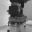
\includegraphics[width=0.99\linewidth]{insertion/robot_view_screenshots/water_target_image1.png}\\
        \centering
    \end{subfigure} \hfill
    \begin{subfigure}[b]{0.20\linewidth}
        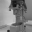
\includegraphics[width=0.99\linewidth]{insertion/robot_view_screenshots/water_target_image2.png}\\
        \centering
    \end{subfigure}     \hfill
    \begin{subfigure}[b]{0.20\linewidth}
        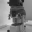
\includegraphics[width=0.99\linewidth]{insertion/robot_view_screenshots/water_target_image3.png}\\
        \centering
    \end{subfigure}  \hfill
    \begin{subfigure}[b]{0.20\linewidth}
        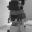
\includegraphics[width=0.99\linewidth]{insertion/robot_view_screenshots/water_target_image4.png}\\
        \centering
    \end{subfigure}    
    \\
    \centering
    \begin{subfigure}[b]{0.40\linewidth}
        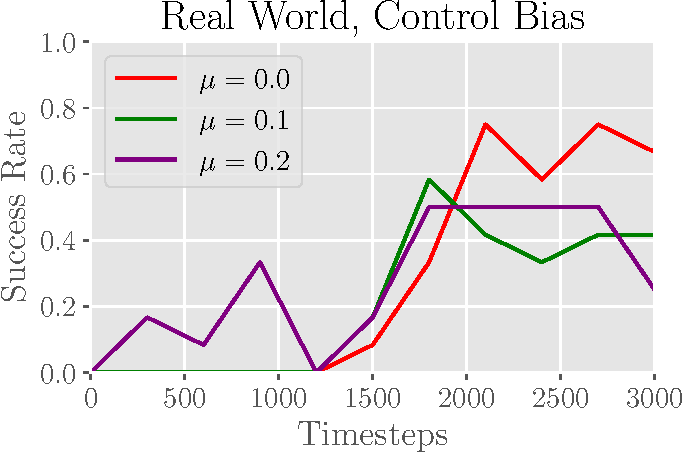
\includegraphics[width=0.99\linewidth]{figs/real_world_control_bias.pdf}\\
        \centering
        (a)
    \end{subfigure} \hfil
    \begin{subfigure}[b]{0.49\linewidth}
        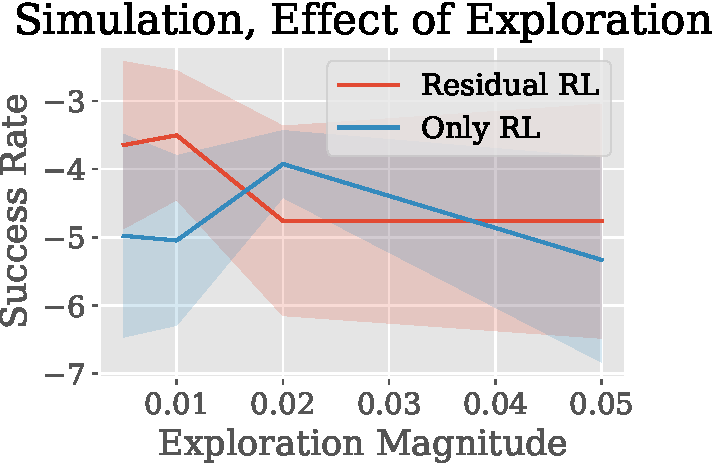
\includegraphics[width=0.99\linewidth]{figs/exploration_noise.pdf}\\
        \centering
        (b)
    \end{subfigure}
    %\includegraphics[scale=1.0]{figurefile}
    \caption{Image-based training using SAC and TD3, together with residual RL and pure RL. The average returns are shown in (a). Plot (b) compares the mean final distance of the image-based training with the dense and sparse setting. }
    \label{image_figure}
    \vspace{15pt}
\end{figure}
\fi


\iffalse
\begin{table}[b!]\label{tab:use_cases}
\centering
\small
\vspace{15pt}
\caption{Evaluation of residual RL on different industrial connectors. }
\renewcommand{\arraystretch}{1.6}
\begin{tabular}{|l|c|c|c|c|l|}
\hline
\multirow{2}{*}{Success rates} & \multirow{2}{*}{P-controller} &  \multirow{2}{*}{Pure RL} &\multicolumn{3}{c|}{Residual RL} \\ \cline{4-6} 
 &  & & Full state & \multicolumn{2}{c|}{Pixels} \\ \hline
USB & 1.0  &  xxx & 0.96  & \multicolumn{2}{c|}{\cellcolor{gray!20} 1.0} \\ \hline
U-sub connector & 0.88 &  xxx &\cellcolor{gray!20} 0.92 & \multicolumn{2}{c|}{0.64} \\ \hline
Waterproof connector & 0.52 &  xxx &0.16 & \multicolumn{2}{c|}{0.48} \\ \hline
\end{tabular}
\vspace{6 pt}
\end{table}
\fi

\iffalse
\begin{figure*}[t]
    \vspace{6pt}
    \centering
    \begin{subfigure}[b]{0.32\linewidth}
        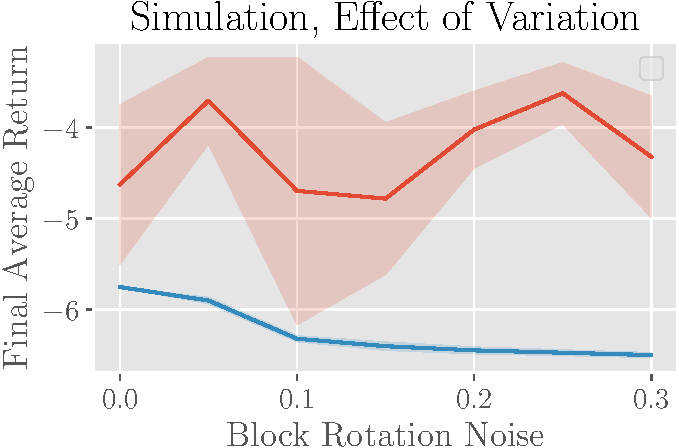
\includegraphics[width=0.99\linewidth]{figs/env_variance_sim.pdf} \\
        \centering
        (a)
    \end{subfigure}
    \begin{subfigure}[b]{0.32\linewidth}
        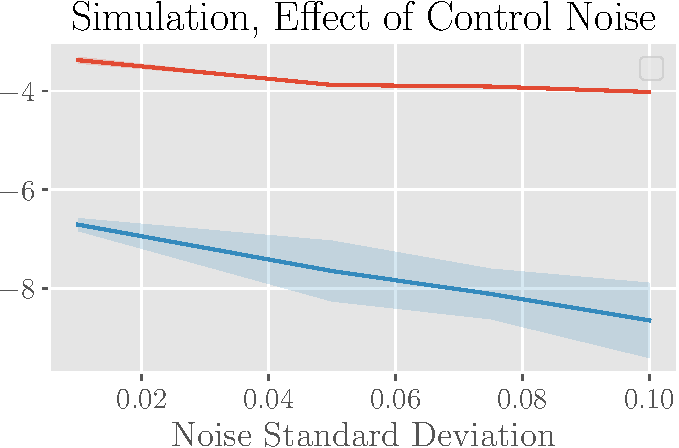
\includegraphics[width=0.99\linewidth]{figs/control_noise_sim.pdf} \\
        \centering
        (b)
    \end{subfigure}
    \begin{subfigure}[b]{0.32\linewidth}
        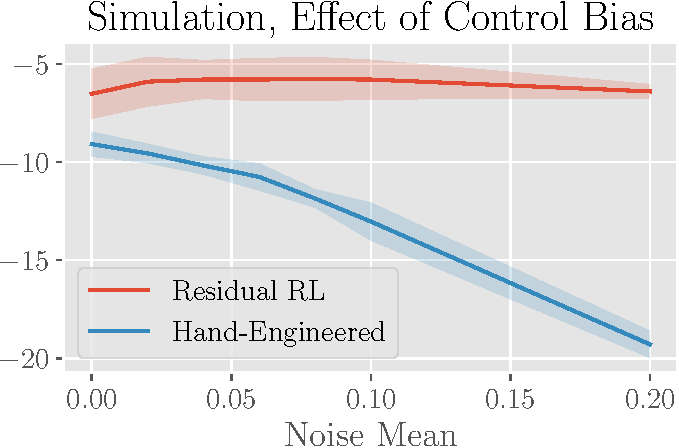
\includegraphics[width=0.99\linewidth]{figs/control_bias_sim.pdf} \\
        \centering
        (c)
    \end{subfigure}
    \caption{Simulation results for different experiments. In each plot, the final average return obtained by running the method for various settings of a parameter is shown. Plot (a) shows that residual RL can adjust to noise in the environment caused by rotation of the blocks in a range of $0$ to $0.3$\,rad. In plot (b), residual RL finds robust strategies in order to reduce the effect of control noise, as the final average return is not greatly affected by the magnitude of noise. Plot (c) shows that residual RL can compensate for biased controllers and maintains good performance as control bias increases, while the performance of the hand-designed controller dramatically deteriorates with higher control bias.} %
    \label{fig:control_bias}
\end{figure*}
\fi


\subsection{Exploration Comparison}
All experiments were also performed using TD3 instead of SAC. 
The final success rates of these experiments are included in Fig.~\ref{fig:tables}. 
When combined with residual RL, SAC and TD3 perform comparably. 
However, TD3 is often substantially less robust.
These results are likely explained by the exploration strategy of the two algorithms. 
TD3 has a deterministic policy and fixed noise during training, so once it observes some high-reward states, it quickly learns to repeat that trajectory. 
SAC adapts the noise to the correct scale, helping SAC stay robust to small perturbations, and because SAC learns the value function for a stochastic policy, it is able to handle some degree of additive noise effectively.
We found that the outputted action of TD3 approaches the extreme values at the edge of the allowed action space, while SAC executed less extreme actions, which likely further improved robustness.


